\documentclass[conference,compsoc]{IEEEtran}

\usepackage{graphicx}
\usepackage{subcaption}
\usepackage{calc}
\def\scalecaption{\normalsize}

\setcounter{figure}{5}

\begin{document}

\begin{figure}[ht]
    \centering
    \begin{subfigure}[b]{1.0\columnwidth}
        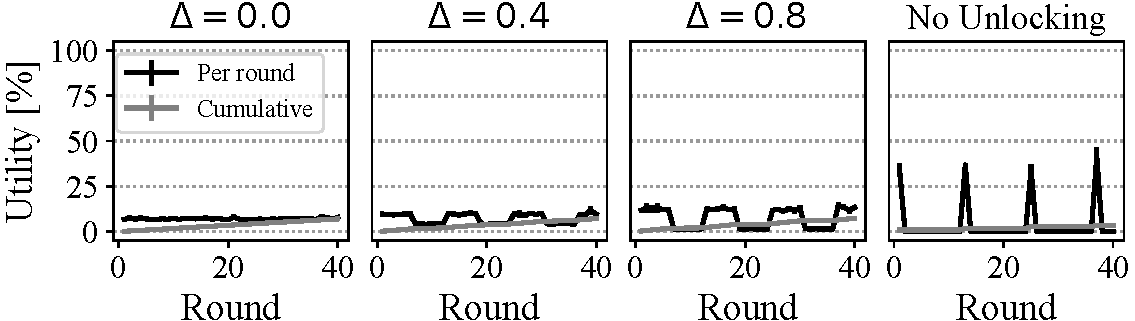
\includegraphics[trim={0 20pt 0 0}, clip, width=1.0\columnwidth]{sp_workloads/sim_round/workloads_round_dpk-gurobi_gm:GM_ncd_woPA}

        \caption{w/o PA}
        \vspace{-3pt}
    \end{subfigure}

    \vspace{10pt}
    \begin{subfigure}[b]{1.0\columnwidth}
        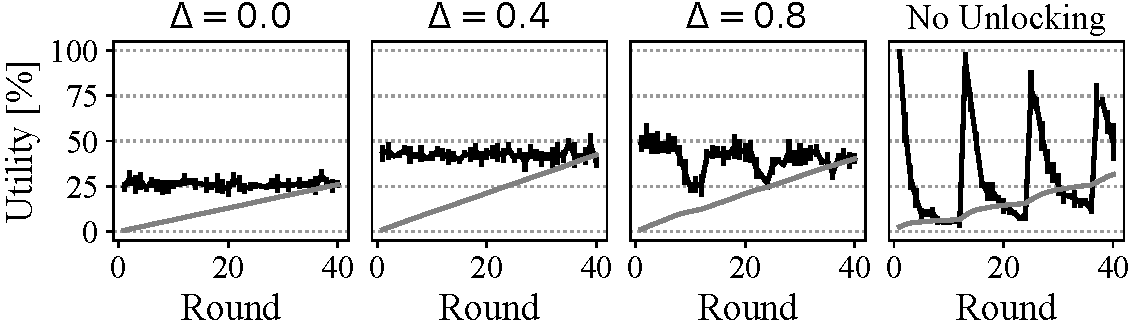
\includegraphics[trim={0 0 0 18pt}, clip, width=1.0\columnwidth]{sp_workloads/sim_round/workloads_round_dpk-gurobi_gm:GM_ncd_wPA}

        \caption{w/ PA}
    \end{subfigure}

    \caption{The effect of budget unlocking on utility per round achieved by the DPK algorithm on the W1:GM workload.}

\end{figure}


\end{document}